\documentclass[a4paper,11pt]{article}
%在此可进行页面设置
%\textwidth=14cm
%\textheight=22cm

\usepackage[33652]{MCMPackage}  %队号在这里填写
%\usepackage[XXX,nosheet]{MCMPackage}%这个参数形式可去掉summary sheet首页。
\problem{A}  %选题

\title{This Is the Article Title}%在此插入论文标题
\date{}

%设置段落之间的距离,若不需要删除或者注释掉latex即可。
\setlength\parskip{.5\baselineskip}

%为了首行缩进
%\usepackage{indentfirst}
%\setlength{\parindent}{2em}

\begin{document}
%摘要
\begin{abstract}
    There is the abstract of our paper. It should be brief enough.\\
    1. "Is" ~~2. ''Is'' ~~3. 'Is'

\end{abstract}
\maketitle%插入标题
\thispagestyle{empty}%本页不遍页码

\newpage%另起一页插入目录
\thispagestyle{empty}%防止目录两页而出现一页带页码
\tableofcontents%目录
\thispagestyle{empty}
\newpage%另起一页书写正文
\pagenumbering{arabic}%开始编页码(阿拉伯数字)

\section{Introduction}
Since the dawn of Industrial Age shed on the human civilization, the life of people has been developed to a large extent in the past two centuries and enjoyed the convenience along with the technology. However, a global problem has emerged, which is bred by the excessive consumption of the resources and irreversible pollution of the environment. It has attracted considerable attention in a variety of organizations and governments and been discussed by the specialists since then. The contradiction of developing economics and protecting nature is a controversial issue, which seems unsolvable.

For meeting human development goals while maintaining the health of ecosystem, the trend of promoting the idea of sustainable development catches on. Sustainable development is an ideal state that living conditions and resource-use continue to meet human needs without undermining the integrity, stability and beauty of the nature. Striving to achieve the sustainable future, various countries has gathered to deliberate specific measures due to their own national conditions.

Comparing to relatively well-rounded developed countries, the implement of developing countries seems more difficult and complex, which may need more time and aids. Loaded with rapid increasing of population, dragged by poor technology and immature management, they need supports and investments from the international organizations. Therefore, it is supposed to set up a scientific and reasonable assessment to estimate the situation of the country and make a practical scheme to allocate their limited resources.

Our work is to build a model to estimate the developing country's need degree of support and intervention according to the analysis of related indicators, then to distinguish the more sustainable countries and policies from the less ones, besides, to predict the change that will occur over the 20 years in the future. In the following parts, we will show the detailed evaluation method and results of 48 Least Developed Countries (LDC), in the end give the prediction of the selected one as an example. %\cite{RefB}.% 引用参考文献

%\subsection{Background}

%\subsection{Our Work}
%这一部分写问题分析以及我们要解决的问题

\section{Assumption}
%这里写模型假设
\begin{enumerate}%[(1)]
\renewcommand{\labelenumi}{(\theenumi)}
    \item Build the co-author network of the Erdos1 authors and analysis of the characteristics of the network.
    \item
\end{enumerate}

\section{Symbol Description}
%符号说明
In the section, we use some symbols for constructing the model as follows.
\begin{center}
\begin{tabular}{c l}%r 表示表格内文本右对齐;c表示居中对齐;l表示左对齐;| 表示竖铅直线
    \toprule[2pt]
    \textbf{Symbol} & \makecell[c]{\textbf{Description}}\\
    \hline
    $\sigma$ & The standard deviation\\
    110010101010 & binary \\
    $\mathbf{F}$ & This is the best beautiful symbol. \\
    \bottomrule[2pt]
    %以下两条指令此处不用
    %\caption{表格标题}
    %\label{标签名}%便于交叉引用
\end{tabular}
\end{center}
P.s:Other symbol instructions will be given in the text.

\section{The Influence of Researchers}%人家论文里这么写的我先这么借鉴过来了
\subsection{Model one:Model abstract}%写下模型的名字,或者描述一下
%具体阐述
%下面示例一个插图
\subsubsection{Insert a picture for example}
In this section,we will test to insert a picture.\\

Look at Figure \ref{fig:1}

\begin{figure}[!h]%[!hptb] !h意思是忽略美学标准,将照片固定到此位置;不会上下浮动% 支持格式eps, pdf, png, jpg
\centering %使得插入的照片居中显示
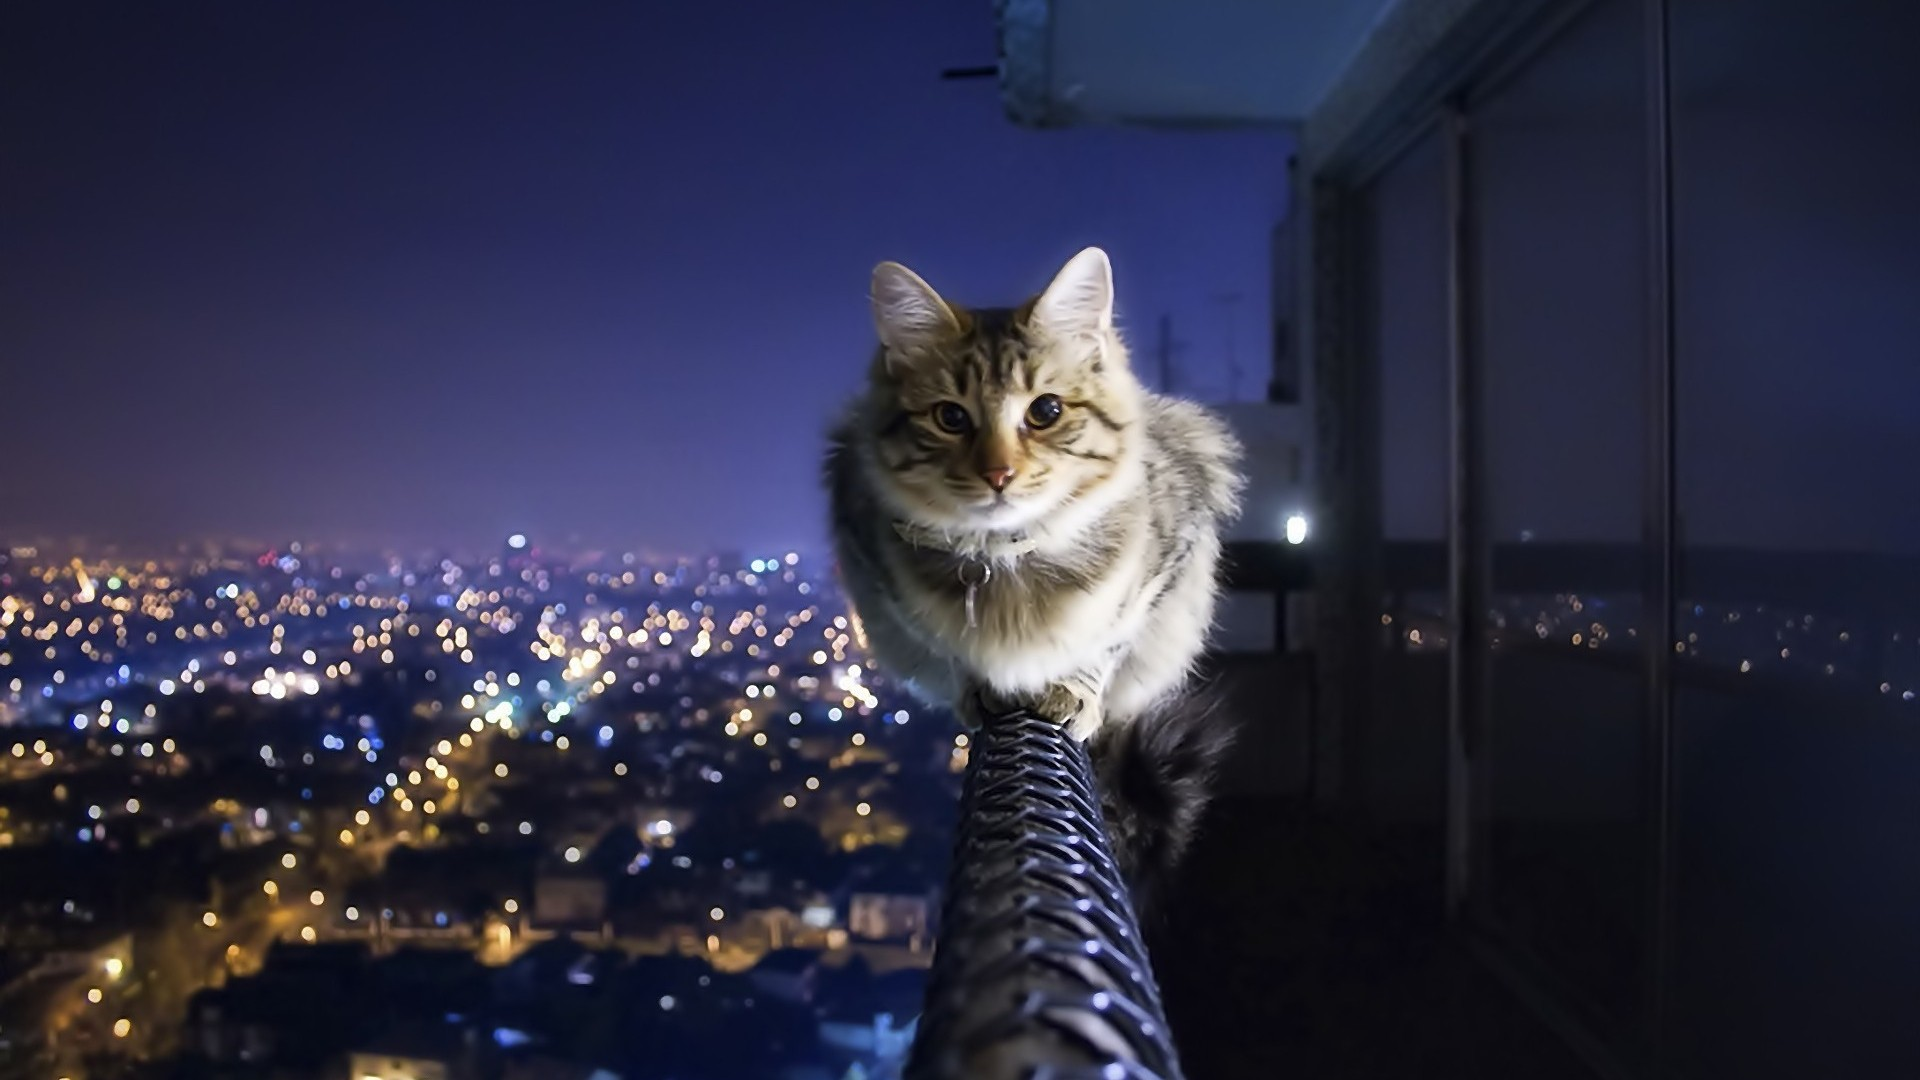
\includegraphics[width=0.50\textwidth]{./Pic/cat.JPG}
% 图片标题
\caption{This is a cat.}
\label{fig:1}       % 给图片一个标签便于交叉引用
\end{figure}

%并列插入图片
\begin{figure}[!h]
  \centering %使得插入的照片居中显示
  \begin{minipage}[t]{.49\linewidth}
   % \framebox{Text}
  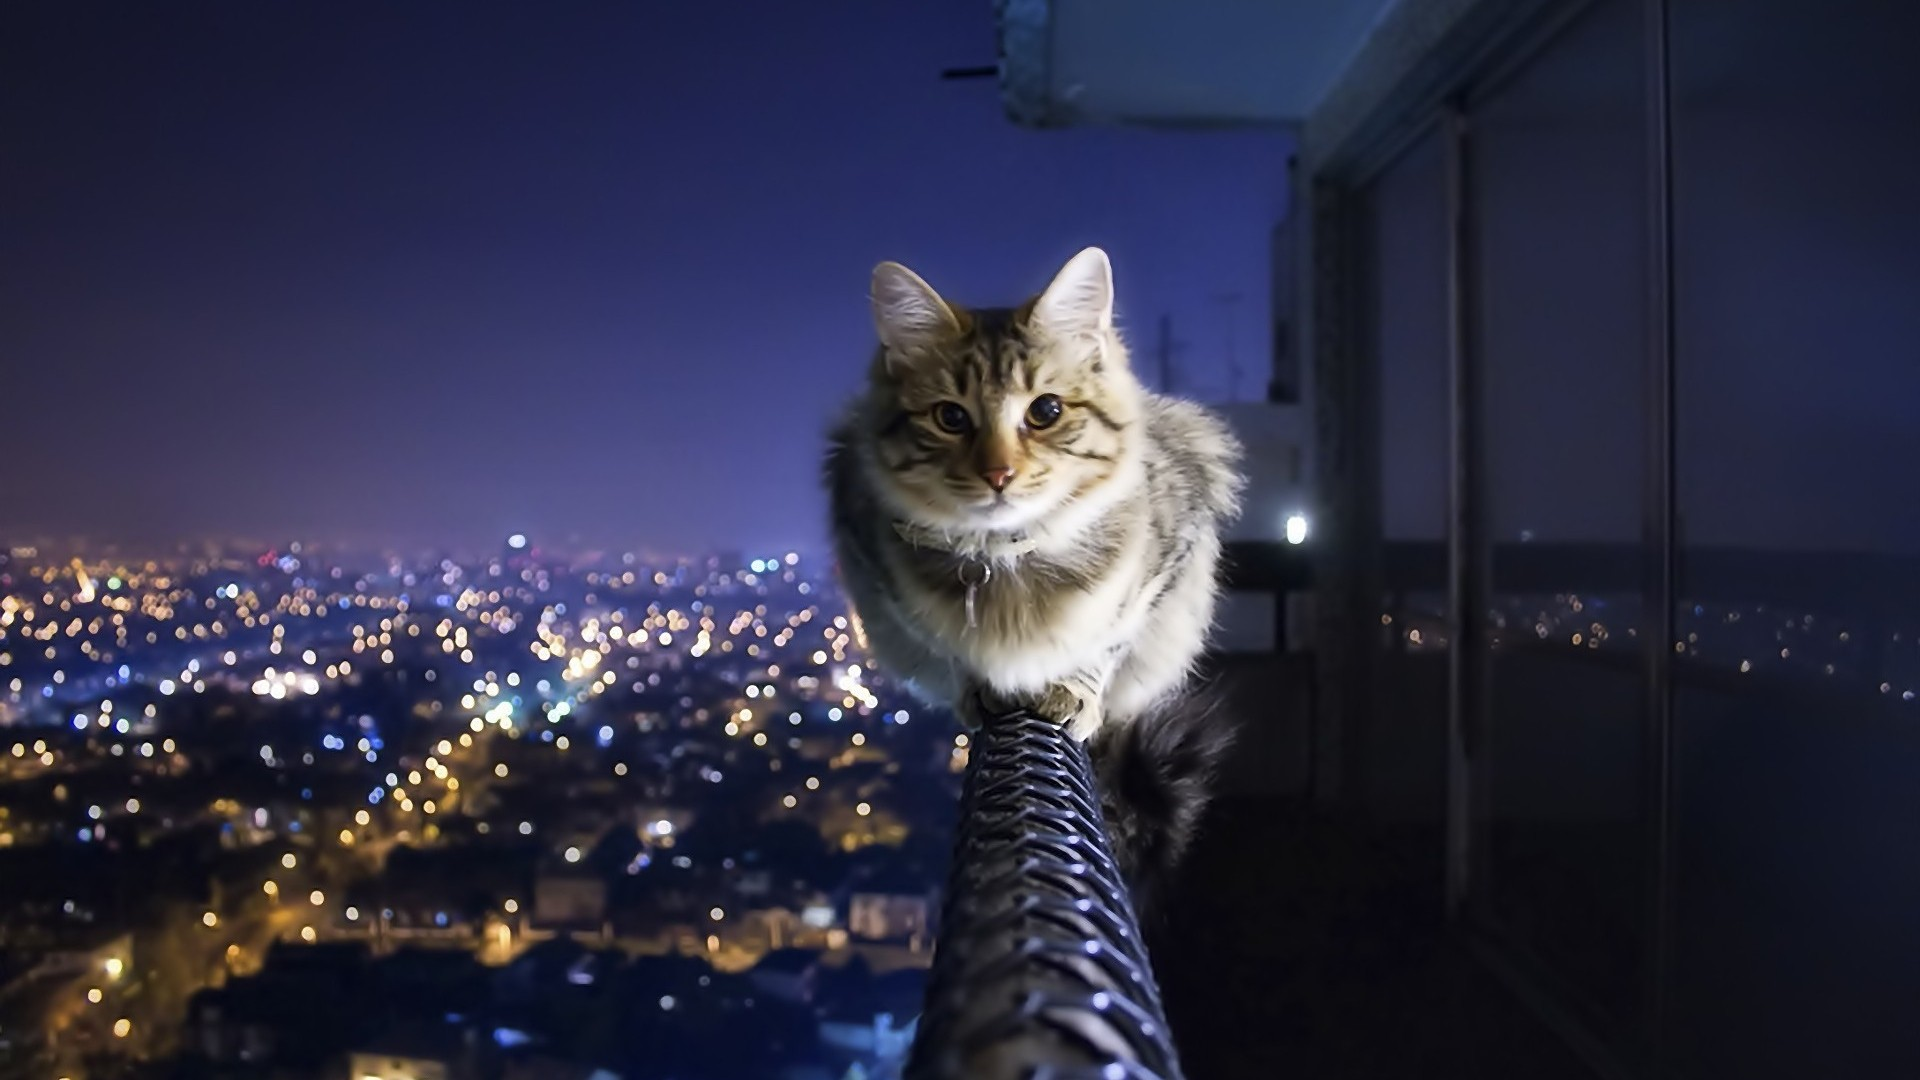
\includegraphics[width=1\textwidth]{./Pic/cat.JPG}
  \caption{This is a cat.}
  \end{minipage}
  \begin{minipage}[t]{.49\linewidth}
  
\includegraphics[width=1\textwidth]{./Pic/human.jpg}
   %\framebox{Text}
  \caption{This is the back of a Human.}
  \end{minipage}
\end{figure}

\subsection{Model two:}

\subsubsection{Test insert math formulas}
In the section, we will insert math formulas.\\
%插入文本中的公式\\
\begin{math}\label{math_1} \ln{(x+1)}+\max{\{\varepsilon,\theta\}} \end{math}\\
%居中并编号的公式\\
\begin{equation}\label{eq:eps} \exists~\delta>0,\quad when \quad |x-x_0|<\delta,\quad s.t.~ |f(x)-f(x_0)|<\varepsilon \end{equation}\\
%居中不编号的公式
\begin{displaymath}\label{math_2} \ln{(x+1)}+\max{\{\varepsilon,\theta\}} \end{displaymath}
\[\ln{(x+1)}+\max{\{\varepsilon,\theta\}}\]%简写形式,同上

\subsubsection{Test Equations}%测试方程组
%这个不加左边的大括号,且每个式子都编号了
\begin{eqnarray}
f(x) & = & \cos x \\
f'(x) & = & -\sin x \\
\int_{0}^{x} f(y)dy & = & \sin x
\end{eqnarray}

\subsubsection{Others}
\[
   \begin{aligned}
   A &= (B + C) + D\\
    &=B + (C + D)\\
   \end{aligned}
\]

OK, let's look at another one.
%这个加了左边的大括号,只有一个编号
\begin{equation}
  \left\{
   \begin{aligned}
   \overset{.}x(t) &=A_{ci}x(t)+B_{1ci}w(t)+B_{2ci}u(t)  \\
   z(t) &=C_{ci}x(t)+D_{ci}u(t) \\
   \end{aligned}
   \right.
\end{equation}

 \[
  A = \left(\begin{array}{ccc}
        a_{11} & a_{12} & a_{13} \\
        a_{21} & a_{22} & a_{23} \\
        a_{31} & a_{32} & a_{33}
      \end{array}\right).
  \]

\subsection{Result Analysis:}

%研究人员综合排名
\begin{table}[!h]%[!hptb]
\centering
\caption{Rank of Researcher (Top 10)}\label{Q2:RankTable For Researcher}%便于交叉引用
\begin{tabular}{c l}
    \toprule[2pt]
    \textbf{Rank} & \makecell[c]{\textbf{Researcher Name}}\\
    \midrule[2pt]
    %\hline
    1 & ALON, NOGA M.\\
    2 & HARARY, FRANK*\\
    3 & GRAHAM, RONALD LEWIS\\
    4 & BOLLOBAS, BELA \\
    5 & RODL, VOJTECH\\
    6 & SOS, VERA TURAN\\
    7 & TUZA, ZSOLT\\
    8 & FUREDI, ZOLTAN\\
    9 & SPENCER, JOEL HAROLD\\
    10 & POMERANCE, CARL BERNARD\\
    \bottomrule[2pt]
\end{tabular}
\end{table}

\section{The Influence of Papers}%同理
%表1:研究人员综合排名
\begin{table}
\centering
\caption{Rank of Researchers' Total Influence (Top 10)}\label{Q2:RankTable For Researcher}% 便于交叉引用
\begin{tabular}{C{3cm} l}
    \toprule[2pt]
    \textbf{Rank} & \makecell[c]{\textbf{Researcher Name}}\\
    \midrule[2pt]
    %\hline
    1 & ALON, NOGA M.\\
    2 & GRAHAM, RONALD LEWIS\\
    3 & RODL, VOJTECH\\
    4 & BOLLOBAS, BELA\\
    5 & HARARY, FRANK*\\
    6 & FUREDI, ZOLTAN\\
    7 & TUZA, ZSOLT\\
    8 & SOS, VERA TURAN\\
    9 & SPENCER, JOEL HAROLD\\
    10 & GYARFAS, ANDRAS\\
    \bottomrule[2pt]
\end{tabular}
\end{table}

\begin{table}[!h]
\centering
\caption{Test}
\begin{tabular}{c | c| >{\columncolor{yellow}}c}
\toprule[1pt]
\diagbox{No.}{Title} & \textbf{L-Title} & \textbf{R-Title}\\
\hline
1 & One & First\\
\cellcolor[rgb]{.9,.9,.9} 2 & Two & Second\\
\cellcolor[rgb]{.2,.9,.9} 3 & Three & Third\\
\bottomrule[1pt]
\end{tabular}
\end{table}

\section{Model Extension}%模型推广

\section{Error/Sensitivity Analysis}%误差/灵敏度分析

\section{Analysis of The Model}% 模型分析


%以下是参考文献
\phantomsection%生成该页的链接
\addcontentsline{toc}{section}{\refname}
\begin{thebibliography}{}
%
% 使用指令\bibitem 构造一条参考文献.
% 具体构造方式,参考以下参考文献格式说明以及示例
% 应尽可能使用英文格式
%
\bibitem{RefJ}
% 期刊引用格式
    % 中文的引用格式
    % 作者. 标题[J].期刊名, 发表年份,  卷号(期号), 页码
    % Author. Article title[J]. Journal name, year, Volume(issue), page numbers.
    % 姓,名字首字母.(年). 题目. 期刊名(斜体), 卷号(期号), 页码.
    Last name, Initials. (year). Title.\emph{The journal name}. Volume(Issue), pages.
    %或者 Last name, Initials.,& Last name, Initials. (year). Title.\emph{The journal name}. Volume(Issue), pages.

\bibitem{RefB}
% 书本/专著引用格式
    % 中文的引用格式
    % 作者名. 书名[M]. 出版地: 出版社, 出版年份: 页码.
    % Author. Book title[M]. Address: Publisher, year: page numbers.
    % 英文引用格式
    % 姓, 名字首字母.(年). 书名(斜体). 出版社所在城市: 出版社.
    Last name, Initials. (year). \emph{Book name}. Address: Publisher.

\bibitem{RefC}
% 文集中的文章
    % 英文引用格式
    % 姓, 名字首字母. (年). 文集名, 文章名(pp.页码). 出版地: 出版社
    Last name, Initials. (year). Collection name, \emph{Article name}(pp.pages). Address: Publisher.

% 学位论文引用格式(英文里等同于专著引用)
\bibitem{RefD}
Author. Article Title[D]. Address: Saver, year: page numbers.
% 网络引用(百科,博客等)
\bibitem{RefI}
The site name, Title. The Site Link. Time.
% 电子文献
\bibitem{RefE}
The main responsibility author. Electronic document titles. Electronic literature source[Symbol]. Site Link, Publish or update date / date references.

% etc
\end{thebibliography}

\begin{appendices}
% 添加多目录
% \include{Appendix1}
% This is Appendix1
% \include{Appendix2}
% This is Appendix2
\section{First appendix}

some text...


Here are simulation programmes we used in our model as follow.\\


\codetitle{Input matlab source:}
\lstinputlisting[language=Matlab]{./code/matlab1.m}


\section{Second appendix}

some more text

\codetitle{Input C++ source:}
\lstinputlisting[language=C++]{./code/sudoku.cpp}
\end{appendices}


\end{document}
